The implementation of the breast cancer detection system was conducted in two parts. The first part corresponds to a common pipeline developed in group, and the second part to individual implementations using the common pipeline as a baseline. The distribution of work during the implementation of the common pipeline can be found in Appendix~\ref{ch:appendix-team-meeting-summaries}.

%%%%%%%%%%%%%%%%%%%%%%%%%%%%%%%%%%%%%%%%%%%%%
%%%%%%%%%%%%%%%%%%%%%%%%%%%%%%%%%%%%%%%%%%%%%
%%%%%%%%%%%%%%%%%%%%%%%%%%%%%%%%%%%%%%%%%%%%%

\section{Common Deep Learning Pipeline}

A detailed flowchart of the deep learning pipeline implemented can be found in  Figure~\ref{fig:implementation-detailed-flowchart}.

\begin{figure}[ht]
\centerline{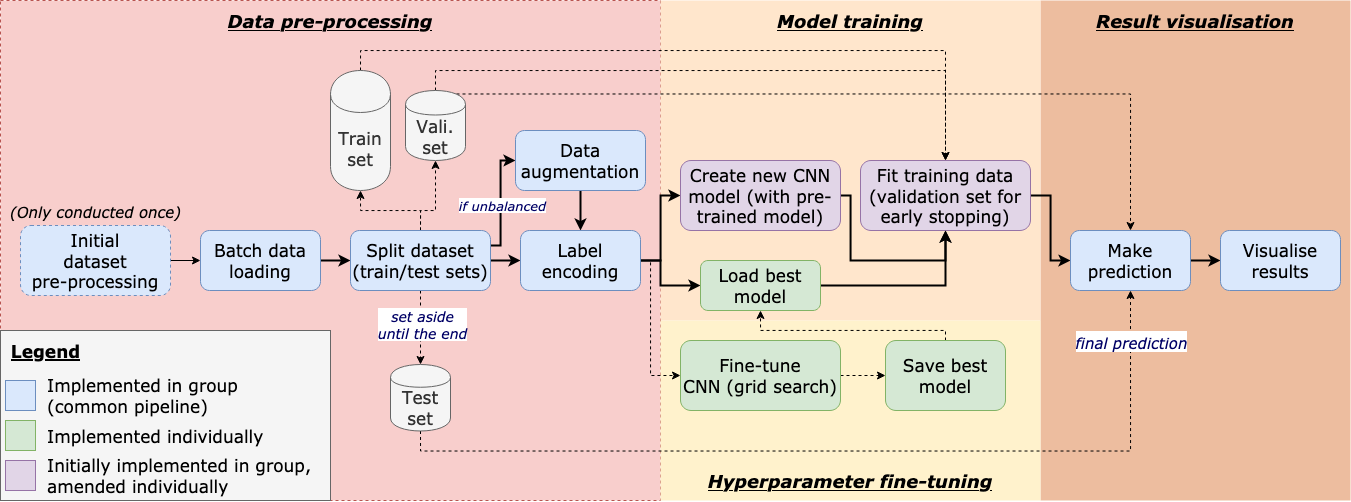
\includegraphics[width=1.25\textwidth]{Dissertation/figures/implementation/detailed flowchart.png}}
\caption{\label{fig:implementation-detailed-flowchart}Flowchart. Created using draw.io.}
\end{figure}

%%%%%%%%%%%%%%%%%%%%%%%%%%%%%%%%%%%%%%%%%%%%%

\subsection{Data pre-processing}

\subsubsection{Processing and organising raw images}

Two Python scripts written to initially parse CSV files mapping image paths and their labels in order to reorganise the images in labelled folders for classification.\\

File formats: PGM and DICOM files converted to arrays to be readable by the CNNs as input.\\

Scikit-Learn's \textit{LabelEncoder} class is used to one-hot encode labels and Keras' \textit{to\_categorical}  function is used to convert to a binary class matrix usable by the CNN models.\\

Data augmentation for the mini-MIAS  dataset images to balance the class distribution. Rotations, noise and rotation flips are randomly added to existing images to create new images.

\subsubsection{Data loading}

Tensorflow cache and batch functions used to load the CBIS-DDSM dataset. No optimisations used for the smaller mini-MIAS dataset (just the Keras \textit{img\_to\_array} and \textit{load\_img} functions).\\

Images resized on import to match the input size of the pre-trained model. For instance, VGG19 takes 224x224px images.\\

Normalising images to fit in [0-1] float range rather than [0-255] integer range.\\

A 60/20/20\% stratified split is used for the mini-MIAS dataset. The Train test split is already done for CBIS-DDSM dataset.

%%%%%%%%%%%%%%%%%%%%%%%%%%%%%%%%%%%%%%%%%%%%%

\subsection{Model training}

A VGG19 pre-trained model (using ImageNet weights) is used through the Keras API. The fully connected layers are replaced with new fully connected layers  to accomodate the breast cancer detection classes (benign and malignant for CBIS-DDSM, and normal as well for mini-MIAS).\\

Training is conducted in two phases:
\begin{itemize}
    \item During the first phase, the VGG19 layers are frozen (weights are not updated during training) and only the fully connected layers are being updated.
    \item Once the first training phase is stopped (using early stopping when the validation loss does not improve after 8 epochs), all the layers are unfrozen and training is resumed at a lower learning rate for the VGG19 models to adapt to the mammograms images.
\end{itemize}

Additional convolution and spooling layers are added before the pre-trained model to accomodate larger images. These are slowly reduced in size as they go through the spooling layers, allowing lower-level features to be learned before passing through the VGG19 model.\\

Once the CNN model is finished training model is saved in HDF5 format in order to save the model's architecture, the layers' hyperparameters, all the connection weights and biases that were learned during training \citep{Geron2019} and the optimiser used.

%%%%%%%%%%%%%%%%%%%%%%%%%%%%%%%%%%%%%%%%%%%%%

\subsection{Results visualisation}

Scikit-Learn's \textit{classification\_report} and \textit{accuracy\_score} functions used to get numerical result metrics.\\

Matplotlib used to plot the ROC curve and seaborn for the confusion matrices.

%%%%%%%%%%%%%%%%%%%%%%%%%%%%%%%%%%%%%%%%%%%%%

\subsection{General}

Python's \textit{argparse} is used to implemenent the CLI application, accepting different arguments such as the dataset to use, the CNN model to use, whether to train or test the model, etc. (see Appendix~\ref{sec:appendix-common-pipeline-instructions}).

The runtime is always measured in seconds to know how long it took to load the data and train the model.

%%%%%%%%%%%%%%%%%%%%%%%%%%%%%%%%%%%%%%%%%%%%%
%%%%%%%%%%%%%%%%%%%%%%%%%%%%%%%%%%%%%%%%%%%%%
%%%%%%%%%%%%%%%%%%%%%%%%%%%%%%%%%%%%%%%%%%%%%

\section{Individual Optimisations}

Regularisation implemented by adding Dropout layers between convolutional layers and fully connected layers.\\

Image sizes of 1024x1024px large used and downscaled using convolutional layers. This size was chosen as it is the size of the mini-MIAS dataset images, which will be used to initially train the CNN before training on the large CBIS-DDSM dataset.\\

Heavy code refactoring, moving every CNN-related code to a custom \textit{CNN\_Model} class for more ease of use and less unnecessary code duplication.